\PassOptionsToPackage{unicode=true}{hyperref} % options for packages loaded elsewhere
\PassOptionsToPackage{hyphens}{url}
%
\documentclass[english,,man,floatsintext]{apa6}
\usepackage{lmodern}
\usepackage{amssymb,amsmath}
\usepackage{ifxetex,ifluatex}
\usepackage{fixltx2e} % provides \textsubscript
\ifnum 0\ifxetex 1\fi\ifluatex 1\fi=0 % if pdftex
  \usepackage[T1]{fontenc}
  \usepackage[utf8]{inputenc}
  \usepackage{textcomp} % provides euro and other symbols
\else % if luatex or xelatex
  \usepackage{unicode-math}
  \defaultfontfeatures{Ligatures=TeX,Scale=MatchLowercase}
\fi
% use upquote if available, for straight quotes in verbatim environments
\IfFileExists{upquote.sty}{\usepackage{upquote}}{}
% use microtype if available
\IfFileExists{microtype.sty}{%
\usepackage[]{microtype}
\UseMicrotypeSet[protrusion]{basicmath} % disable protrusion for tt fonts
}{}
\IfFileExists{parskip.sty}{%
\usepackage{parskip}
}{% else
\setlength{\parindent}{0pt}
\setlength{\parskip}{6pt plus 2pt minus 1pt}
}
\usepackage{hyperref}
\hypersetup{
            pdftitle={Non-word repetition in Yélî Dnye},
            pdfauthor={Alejandrina Cristia~\& Marisa Casillas},
            pdfkeywords={phonology, non-word repetition, development},
            pdfborder={0 0 0},
            breaklinks=true}
\urlstyle{same}  % don't use monospace font for urls
\usepackage{graphicx,grffile}
\makeatletter
\def\maxwidth{\ifdim\Gin@nat@width>\linewidth\linewidth\else\Gin@nat@width\fi}
\def\maxheight{\ifdim\Gin@nat@height>\textheight\textheight\else\Gin@nat@height\fi}
\makeatother
% Scale images if necessary, so that they will not overflow the page
% margins by default, and it is still possible to overwrite the defaults
% using explicit options in \includegraphics[width, height, ...]{}
\setkeys{Gin}{width=\maxwidth,height=\maxheight,keepaspectratio}
\setlength{\emergencystretch}{3em}  % prevent overfull lines
\providecommand{\tightlist}{%
  \setlength{\itemsep}{0pt}\setlength{\parskip}{0pt}}
\setcounter{secnumdepth}{0}
% Redefines (sub)paragraphs to behave more like sections
\ifx\paragraph\undefined\else
\let\oldparagraph\paragraph
\renewcommand{\paragraph}[1]{\oldparagraph{#1}\mbox{}}
\fi
\ifx\subparagraph\undefined\else
\let\oldsubparagraph\subparagraph
\renewcommand{\subparagraph}[1]{\oldsubparagraph{#1}\mbox{}}
\fi

% set default figure placement to htbp
\makeatletter
\def\fps@figure{htbp}
\makeatother

\usepackage{fontspec}

\setmainfont{Doulos SIL} % Set main font to Doulos SIL
\ifnum 0\ifxetex 1\fi\ifluatex 1\fi=0 % if pdftex
  \usepackage[shorthands=off,main=english]{babel}
\else
  % load polyglossia as late as possible as it *could* call bidi if RTL lang (e.g. Hebrew or Arabic)
  \usepackage{polyglossia}
  \setmainlanguage[]{english}
\fi

\title{Non-word repetition in Yélî Dnye}
\author{Alejandrina Cristia\textsuperscript{1}~\& Marisa Casillas\textsuperscript{2}}
\date{}

\authornote{All data are made available in a repository in the Open Science Framework. AC acknowledges the support of the Agence Nationale de la Recherche (ANR-17-CE28-0007 LangAge, ANR-16-DATA-0004, ANR-14-CE30-0003, ANR-17-EURE-0017); and the J. S. McDonnell Foundation Understanding Human Cognition Scholar Award.

Correspondence concerning this article should be addressed to Alejandrina Cristia, 29, rue d'Ulm, 75005 Paris, France. E-mail: \href{mailto:alecristia@gmail.com}{\nolinkurl{alecristia@gmail.com}}}

\abstract{
In nonword repetition (NWR) studies, participants are presented auditorily with an item that is phonologically legal but lexically meaningless in the local language. NWR scores are thought to reflect long-term phonological knowledge as well as online phonological working memory and flexible production patterns. In this study, we report on NWR results among children learning Yêly Dnyé, an isolate spoken in Rossel Island, PNG, with an unusually dense phonological inventory. This study contributes to three lines of research. First, we document that non-word items containing typologically rare sounds are repeated without changes less often that non-words containing more common sounds. Second, we document rather weak effects of item length, contributing to other research suggesting that length effects may be language-specific. Third, we do not find strong individual variation effects in this population, contrary to previous results documenting strong age-related effects. Together, these data provide a unique view of online phonological processing in a seldom-studied language, and contribute to both typological and language acquisition research.


}

\begin{document}
\maketitle

\hypertarget{todo-middy}{%
\subsection{TODO Middy}\label{todo-middy}}

\begin{itemize}
\tightlist
\item
  look through this manuscript for bits of text to be written by \textbf{mc}
\item
  double check demo -- probably start with the xlsx version that has the children's first names, date of birth, and date of test. I looked again at my local files (still haven't checked the labs' ones) and I'm surprised I have maternal education for more children than I have birth order for\ldots{} If you correct this, to generate the csv I also round the age, assign age.rounded to reported age (in years) when DOB is missing, remove first names, DOB, DOTest and age.precise before pushing to github
\item
  double check my frequency entries in segments.xlsx using the search function in \url{https://phoible.org/parameters}; take a look at \url{http://phoible.github.io/conventions/} in case you see something about double articulation (I didn't find tp or lBj)
\item
  double check also stim\_seg\_freq -- why are some items still with NA freq?
\item
  draft discussion
\end{itemize}

\hypertarget{todo-alex}{%
\subsection{TODO Alex}\label{todo-alex}}

\begin{itemize}
\tightlist
\item
  add information about proportion of mispronunciations that are real based on other papers
\item
  add effect sizes to all analyses
\item
  ? correct treatment of words whose mispronunciation is an English word:
  mispronunciation meaning
  361 two two
  362 two two
  879 no-pinêt English: no peanut
  908 nodedi English: no daddy
  933 no--dadi English: no daddy
  949 petrumi English: ``true''
  950 petrumi English: ``true''
  951 petrumi English: ``true''
  1373 wee English: where
  1374 wee English: where
  1375 wee English: where
  1379 wee English: where
  1380 wee English: where
  1388 wee English: where
  1394 wee English: where
  1396 wee English: where
  1398 wee English: where
  1399 wee English: where
  1402 wat English: what
  1405 wat English: what
  1411 wee English: where
\end{itemize}

\hypertarget{introduction}{%
\subsection{Introduction}\label{introduction}}

Although infants begin to learn about their native language's phonology within the first year, many studies suggest that in perception and production, in phonetics and phonology, their knowledge continues to develop throughout childhood (e.g., Hazan \& Barrett, 2000). One common task in this line of research is nonword repetition (NWR). In NWR studies, participants are presented auditorily with an item that is phonologically legal but lexically meaningless in the language children are learning. The child should immediately try to say it back without changing anything. NWR scores are thought to reflect long-term phonological knowledge (which allows the child to perceive the item precisely even though it is not a real word they have encountered before) as well as online phonological working memory (to encode the item in the interval between hearing it and saying it back) and flexible production patterns (to produce the item precisely even though it had never been pronounced before).

NWR has been used to seek answers to a variety of theoretical questions, including what the links between phonology, working memory, and the lexicon are (Bowey, 2001), and to assess the extent to which apparent phonological constraints found in the lexicon affect online production (Gallagher, 2014). It is also frequently used for applications, notably as a diagnostic for language delays and disorders (Estes, Evans, \& Else-Quest, 2007). Since non-words can be generated in any language, it has attracted the attention of researchers working in multilingual and linguistically diverse environments, particularly in Europe (Action, 2009; Meir, Walters, \& Armon-Lotem, 2016). However, it has been seldom used outside of Europe and North America (with exceptions including Gallagher, 2014, and Cristia, Farabolini, Scaff, Havron, and Stieglitz (2020)).

In this study, we report on NWR results among children learning Yêly Dnyé, an isolate spoken in Rossel Island, PNG, with an unusually dense phonological inventory. The present report uses these unique data to contribute to several lines of research. First, we made sure that some of the non-word items contained typologically rare and/or challenging sounds, so that we can contribute to the study of whether rare sounds are disadvantaged in perception and/or production, both in terms of overall repetition scores and patterns of mispronunciation. Second, we look at the effects of item length, since previous NWR research has uncovered variable effects. Third, we contribute to the basic NWR literature by adding a data point for children learning a rarely-studied language and culture, and further investigating whether there are structured sources that account for individual variation.

\hypertarget{yuxe9luxee-dnye-phonological-overview}{%
\subsubsection{Yélî Dnye phonological overview}\label{yuxe9luxee-dnye-phonological-overview}}

Yélî Dnye is an isolate language (presumed Papuan) spoken by approximately 7,000 people residing on Rossel Island, which is found at the far end of the Louisiade Archipelago in Milne Bay Province, Papua New Guinea. The Yélî sound system, much like its baroque grammatical system (Levinson, n.d.), is unlike any other in the region.

With only four primary places of articulation (bilabial, alveolar, post-alveolar, and velar) and no voicing contrasts, the phonological inventory is remarkably packed with acoustically similar segments. The core oral stop set includes both singleton (/p/, /t/, /ṭ/, and /k/) and doubly-articulated (/tp/, /ṭp/, /kp/) segments, with full nasal equivalents (/m/, /n/, /ṇ/, /ŋ/, /nm/, /ṇm/, /ŋm/), and with a substantial portion of these able to be contrastively pre-nasalized or nasally released (/mp/, /nt/, /ṇṭ/, /ŋk/, /nmtp/, /ṇmṭp/, /ŋmkp/, /ṭṇ/, /kŋ/, /ṭpṇm/, /kpŋm/). A large number of this combinatorial set can further be contrastively labialized or palatalized on release, or both (e.g., /pʲ/, /pʷ/, /pʲʷ/; /tpʲ/; /ṇmḍbʲ/; see Levinson (n.d.) for details). The consonantal inventory also includes a number of non-nasal continuants (/w/, /j/, /ɣ/, /l/, /βʲ/, /lʲ/, /lβʲ/). Vowels in Yélî Dnye may be oral or nasal, short or long. The 10 oral vowel qualities, which span four levels of vowel height, (/i/, /ɯ/, /u/, /e/, /o/, /ə/, /ɛ/, /ɔ/, /æ/, /ɑ/) can be produced as short or long vowels, with 7 of these able to appear as short and long nasal vowels as well (/i/, /u/, /ə/, /ɛ/, /ɔ/, /æ/, /ɑ/).

In total, Yélî Dnye uses 90 distinctive segments (93 when including consonants that are extremely rarely used), far outstripping the phonemic inventory size of other documented Papuan languages (Levinson (n.d.); Foley 1986) and includes at least two contrasts not yet been documented elsewhere {[}labial-coronal double-articulations with dental vs.~post-alveolar coronal placement in both oral and nasal stops, Maddieson \& Levinson 2001; Ladefoged and Maddieson 1996{]}.

Most words in Yélî Dnye are bisyllabic (\textasciitilde{}50\%), with monosyllabic words (\textasciitilde{}40\%) appearing most commonly after that, and with tri-and-above syllabic words appearing least frequently (\textasciitilde{}10\%; based on \textgreater{}5800 lexemes in the current Yélî Dnye dictionary, Levinson, n.d.). The vast majority of syllables use a CV format. A small portion of the lexicon features words with a final closed syllable, limited to codas of -/m/, -/p/, or -/j/ (e.g., `ndap' (Spondylus shell) /ṇṭæp/). However, in spontaneous speech an epenthetic /ɯ/ is often inserted after word-final coda, yielding a CVCV structure instead (e.g., `ndapî' /`ṇṭæ.pɯ/). This process is used frequently with English loan words that have a coda (e.g., 'ponî' (phone) /`pɔ.nɯ/). An even smaller portion of the lexicon features words starting with a vowel (e.g., 'ala' (here) /æ.'læ/), but these are limited to /æ/-. Finally, the lexicon features a handful of single-vowel grammatical morphemes (see Levinson (n.d.) for details).

While all consonants can appear in the first syllable of the word, the second syllable onset consonant in bisyllabic roots is almost exclusively drawn from a subset of the simplex consonants (in order of descending frequency: /m/, /ṭ/, /n/, /p/, /l/, /w/, /j/, /pʷ/, /ŋ/, /k/, /t/, /ɣ/, /mʷ/). In monosyllabic stems, oral vowels (short: 43\% and long: 31\%) are more common than nasal ones (short: 4\% and long: 22\%), with the first syllable of bisyllabic stems following a similar pattern. Most vowels in the second syllable of bisyllabic stems are also short and oral, with a potential preference for rounding harmony between the first and second vowels. Stress typically falls on the first syllable of bisyllabic words, on the first and third syllables of tetrasyllabic words, and on the first or second syllable of trisyllabic words, depending on its vocalic features (see Levinson (n.d.) for details).

\hypertarget{the-yuxe9luxee-community}{%
\subsubsection{The Yélî community}\label{the-yuxe9luxee-community}}

The current study also contributes to increasing the cultural diversity of the populations for which NWR data have been collected. As mentioned previously, this method has been used almost exclusively in urban, industrialized populations, with only one exception to our knowledge (Cristia et al., 2020). We therefore provide some background information tol help understand some aspects of our study, including the estimation of children's ages and the relationship between NWR scores and children's demographic characteristics.

Most speakers of the language grow up speaking it monolingually until they begin attending school around the age of 7;
school instruction is in English. While monolingual Yélî Dnye upbringing is common, multilingual families are not unusual, particularly in the region around the Catholic Mission---the same region in which the current data were collected---, where there is a higher incidence of married-in mothers from other islands (Brown \& Casillas, n.d.). Children in these multilingual families grow up speaking Yélî Dnye and English, Tok Pisin, and/or some other language(s) from the region.

Most Yélî people are swidden horticulturalists, raising a variety of tubers (e.g., yams, manioc, taro), coconut, banana, and more in their gardens. In addition to garden foods, Yélî children grow up eating fish and foraging for shellfish and nuts, which provide a regular source of extra protein. The typical household in our dataset includes seven individuals and is situated among a collection of 4 or more other households, with structures often arranged around an open grassy area. These household clusters are organized by patrilocal relation, such that they typically comprise a set of brothers, their wives and children, and their mother and father, with neighboring hamlets also typically related through the patriline.

Laying 250 nautical miles off the coast of mainland PNG and surrounded by barrier reef, transport to and from the island is both infrequent and irregular. There is no electricity system (we use solar panels) or motor vehicles on the island, save dinghys with outboard motors that are primarily reserved for medical transport, when there is deisel available. There is a medical radio connection at the health clinic (at the Catholic mission) via which news and messages are often passed along. There is also a cellular tower on the island, though it is typically not functioning. As such, access to news and outside resources, particularly international connections and larger data transfers, is typically unavailable. Our data collection is therefore limited to the duration of the researchers' on-island visits.

Despite restricted outside contact, formal education is a priority for many Yélî families. A recent study surveying more than 40 parents of young children in this region of the island found that nearly all parents completed 6 or more years of education, with 65\% of mothers and 49\% of fathers completing the full range of locally available education (\textasciitilde{}9 years), with around half of those parents having pursued an additional 2+ years of education on other islands in the region or on mainland PNG (Casillas, Brown, \& Levinson, 2020). While there are a handful of local schools around the island, these may be well out of walking distance for many children (i.e., more than 1 hour on foot or by canoe each day), and so it is very common for households to billet school children during the weekdays for months at a time (or for whole months if the child's home is very far). Combined with practices of collective child guardianship within their close-knit hamlets, the practical outcome for researchers is that adult consent can often come from a combination of aunts, uncles, adult cousins, and grandparents standing in for the child's parents---to this child assent is also culturally pertinent, as child independence is encouraged and respected from toddlerhood onward (Brown \& Casillas, n.d.).\footnote{Note that in a few cases this does mean that precise details such as child date of birth, parent age in years, and parent education was only able to be approximated as the parents were residing on another part of the island.} Finally, as mentioned, the language of schooling in this region is English, and so the majority of teens and adults on the island speak some English---many speak it very fluently.

While work on Yélî language development is growing (e.g., Brown, 2011, 2014; Brown \& Casillas, n.d.; Casillas et al., 2020; Liszkowski, Brown, Callaghan, Takada, \& de Vos, 2012), our knowledge of children's linguistic development is quite limited, and research into their phonological development in particular has only just begun {[}e.g., Bram's thesis; MC's CFH data{]}. What we do know about the early language environment is that, while child-directed speech is relatively infrequent throughout the day (Casillas et al., 2020), shared caregiving practices and a near-universal fondness for social interaction with young children ensure that speech directed to children comes from all types of speakers: women, men, and other children (Bunce et al., n.d.; Casillas et al., 2020). While speech from women predominates in young children's speech environments on Rossel, as it does elsewhere (Bergelson et al., 2019; Bunce et al., n.d.), there is a significant and marked increase in child-directed speech from other children as infants get older (Bunce et al., n.d.; Casillas et al., 2020). This increase in child-directed speech from other children is attributed to the fact that, starting around age 2, children often spend large swaths of the day playing, swimming, and foraging for fruit, nuts, and shellfish in large (\textasciitilde{}10 people) independent and mixed-age child play groups (Brown \& Casillas, n.d.; Casillas et al., 2020).

\hypertarget{brief-review-of-nwr-for-our-purposes}{%
\subsubsection{Brief review of NWR for our purposes}\label{brief-review-of-nwr-for-our-purposes}}

The basic structure of NWR involves the participant hearing a non-word, like ``bilik'', which they need to repeat back without changing anything that is contrastive in the language. For instance, in English, a response of ``bilig'' or ``pilik'' will be scored as incorrect; a response ``biilik'', where the vowel is lengthened without change of quality would be scored as correct, because English does not have a pure length contrast.

Aside from this central basic structure, there is some variation in the presentation procedure and structure of items found in previous NWR work. For example, items are often presented orally by the experimenter (Torrington Eaton, Newman, Ratner, \& Rowe, 2015), although an increasing number of studies have turned to playing back the stimuli in order to have greater control of the stability of the presentation (Brandeker \& Thordardottir, 2015). Additionally, while some studies have used 10-15 non-words, others have employed up to 46 unique items (Piazzalunga, Previtali, Pozzoli, Scarponi, \& Schindler, 2019). Often, authors modulate structural complexity, typically measured in terms of item length (measured in number of syllables) and/or syllable structure (open as opposed to closed syllables, Gallon, Harris, \& Van der Lely, 2007).

Previous work seems to avoid difficult sounds, but we felt this was important to represent Yélî Dnye, so we also varied this factor. We designed a relatively large number of items but, aware that this may render the task longer and more tiresome, we split some of the items across children. This allowed us to get NWR scores for more items.

Naturally, designing the task in this way may render the study of individual variation within the population more difficult because different children are exposed to different items. However, a review of previous work on individual variation suggested to us that effects of individual differences are relatively small, and would not be detectable with the sample size that we could collect in a given visit.

That said, we contribute to the literature by also reporting descriptive analyses of individual variation that could potentially be integrated in meta-analytic efforts. Based on previous work, we looked at potential improvements with age (Farmani et al., 2018; Kalnak, Peyrard-Janvid, Forssberg, \& Sahlén, 2014; Vance, Stackhouse, \& Wells, 2005), and potential negative effects of bilingual exposure (Brandeker \& Thordardottir, 2015; Meir \& Armon-Lotem, 2017; Meir et al., 2016). Previous work typically finds no significant differences as a function of maternal education (e.g., Farmani et al., 2018; Kalnak et al., 2014; Meir \& Armon-Lotem, 2017) or child gender (Chiat \& Roy, 2007). Although past research has not often investigated potential effects of birth order on NWR, there is a sizable literature on these effects in other language tasks (Havron et al., 2019), and therefore we report on those too.

\hypertarget{research-questions}{%
\subsubsection{Research questions}\label{research-questions}}

After some preliminary analyses to set the stage, we address the following questions:

\begin{itemize}
\tightlist
\item
  Does the frequency of sounds across languages predict NWR? Are rarer sounds more often substituted by commoner sounds?
\item
  How does score change as a function of item length in number of syllables?
\item
  Is individual variation attributable to child age, sex, birth order, monolingual status, and/or parental education?
\end{itemize}

In view of the hypothesis-driven nature of this work, we had considered boosting the interpretational value of this evidence by announcing our analysis plans prior to conducting them. However, we realized that even pre-registering an analysis would be equivocal because we do not have enough power to look at all relationships of interest, and often to detect any of the known effects given their variability across studies. To illustrate this, we portray studies in which children's NWR scores were gathered between 4 and 12 years of age, and reported separately for items that are relatively short (1-2 syllables) versus longer items (3-4 syllables) in Figure 1. Notice that the effect of stimulus length is minuscule among Italian children (Piazzalunga et al., 2019), but considerable among Tsimane' children (Cristia et al., 2020), where a drop of 40 percentage points is observed at all ages. A similar difference in NWR scores for short versus long items was observed among Arabic children (Jaber-Awida, 2018). Even the effect of age is unstable in this sample. Whereas it is quite clear that children's NWR scores increase in the Italian data, age effects are less stable among Tsimane' children. Therefore, all analyses here are descriptive and should be considered exploratory.

\begin{figure}
\centering
\includegraphics{manuscript_files/figure-latex/prevlit-fig-1.pdf}
\caption{\label{fig:prevlit-fig}NWR scores as a function of age (in years) and item length for comparable studies. Arabic data from Jaber et al. (2018); Italian data from Piazzalunga et al. (2019); Tsimane' from Cristia et al. (2020); Yélî data from the present study.}
\end{figure}

\hypertarget{methods}{%
\subsection{Methods}\label{methods}}

\hypertarget{stimuli}{%
\subsubsection{Stimuli}\label{stimuli}}

Many NWR studies are based on a fixed list of 12-16 items that vary in length between 1 and 4 syllables, often additionally varying syllable complexity and/or cluster presence and complexity, always meeting the condition that they do not mean anything in the target language (e.g., Balladares, Marshall, \& Griffiths, 2016; Wilsenach, 2013). We kept the same variation in item length and the non-meaningfulness requirement, but we did not vary syllable complexity and clusters because these are vanishingly rare in Yély Dnye. We also increased the number of items an individual child would be tested on, so that a child would get up to 23 items to repeat (note that up to other work has also used 24-30 items: Jaber-Awida, 2018; Kalnak et al., 2014), and we created more items and distributed them across children, so as to increase the coverage, and be able to study more items.

A first list of candidate items was generated in 2018 by selecting simple consonants (``p'', ``t'', ``d'', ``k'', ``m'', ``n'', ``w'', ``y'') and vowels (``i'', ``o'',``u'', ``a'',``e'') that were combined into consonant-vowel syllables, further sampling the space of 1- to 4-syllable sequences. These candidates were automatically checked against Levinson's 2015 dictionary and removed from consideration if they appeared in the dictionary. The second author presented them orally to three local research assistants, who were asked to repeat them and further say whether they were real words. Any item for which two or more of the assistants reported them having a meaning or some form of association was excluded.

A second list of candidate items was generated in 2019 by selecting complex consonants and systematically crossing them with all the vowels in the Yélî inventory to produce consonant-vowel monosyllables. As before, items were automatically excluded if they appeared in the dictionary. Additionally, since hearing vowel length in monosyllables in isolation is challenging, any item that had a short/long real word neighbor was filtered out. Since the phonology and phonetics of Yélî is still in the process of being described (Levinson, n.d.), there could have been undocumented constraints that rendered items illegal. Therefore, we made sure that the precise consonant-vowel sequence occurred in some real word in the dictionary (i.e., that there was a longer word included the monosyllable as a subsequence). These candidates were presented to one informant, for a final check that they did not mean anything. Together with the 2018 selection, they were recorded using a headset \textbf{XXX }mc** please fill in** and an Olympus \textbf{XXX }mc** please fill in** from the written form presented together with the same item orally (by the second author). The complete recorded list was finally presented to two more informants, who could repeat all the items and who confirmed there were no real words. Even so, there was one monosyllable that was often identified as a real word (intended ``yî'' /yXX/; identified as ``yi'' /yi/, \emph{tree}). This item is removed from analyses below.

The final list is composed of three practice items; 20 monoysllables containing sounds that are less frequent in the world's languages than singleton plosives; 8 bisyllables; 12 trisyllables; and 4 quadrisyllables (see Table 2).

\begin{table}

\caption{\label{tab:tab2-stims}NWR stimuli in orthographic and phonological representations.}
\centering
\begin{tabular}[t]{llllllllll}
\toprule
\multicolumn{2}{c}{Practice} & \multicolumn{2}{c}{Monosyll} & \multicolumn{2}{c}{Bisyll} & \multicolumn{2}{c}{Trisyll} & \multicolumn{2}{c}{Tetrasyll} \\
\cmidrule(l{3pt}r{3pt}){1-2} \cmidrule(l{3pt}r{3pt}){3-4} \cmidrule(l{3pt}r{3pt}){5-6} \cmidrule(l{3pt}r{3pt}){7-8} \cmidrule(l{3pt}r{3pt}){9-10}
Orth. & Phon. & Orth. & Phon. & Orth. & Phon. & Orth. & Phon. & Orth. & Phon.\\
\midrule
nopimade & nɔpimæṭɛ & dp:a & ṭp̃æ & kamo & kæmɔ & dimope & ṭimɔpɛ & dipońate & ṭipɔnætɛ\\
poni & pɔni & dpa & ṭpæ & kańi & kæni & diyeto & ṭijɛtɔ & ńomiwake & nɔmiwækɛ\\
wî & wɯ & dpâ & ṭpɑ & kipo & kipɔ & meyadi & mɛjæṭi & todiwuma & tɔṭiwumæ\\
 &  & dpê & ṭpə & ńoki & nɔki & mituye & mitujɛ & wadikeńo & wæṭikɛnɔ\\
 &  & dpéé & ṭpeː & ńomi & nɔmi & ńademo & næṭɛmɔ &  & \\
\addlinespace
 &  & dpi & ṭpi & piwa & piwæ & ńayeki & næjɛki &  & \\
 &  & dpu & ṭpu & towi & tɔwi & ńuyedi & nujɛṭi &  & \\
 &  & gh:ââ & ɣ̃ɑː & tupa & tupæ & pedumi & pɛṭumi &  & \\
 &  & ghuu & ɣuː &  &  & tiwuńe & tiwunɛ &  & \\
 &  & kp:ââ & kp̃ɑː &  &  & tumowe & tumɔwɛ &  & \\
\addlinespace
 &  & kpu & kpu &  &  & widońe & wiṭɔnɛ &  & \\
 &  & lv:ê & lβʲ̃ə &  &  & wumipo & wumipɔ &  & \\
 &  & lva & lβʲæ &  &  &  &  &  & \\
 &  & lvi & lβʲi &  &  &  &  &  & \\
 &  & tp:a & tp̃æ &  &  &  &  &  & \\
\addlinespace
 &  & tpâ & tpɑ &  &  &  &  &  & \\
 &  & tpê & tpə &  &  &  &  &  & \\
\bottomrule
\end{tabular}
\end{table}

A Praat script was written to randomize this list 20 times, and split it into two sublists, to generate 40 different elicitation sets. The 40 elicitation sets are available online from \url{https://osf.io/5qspb}. The split had the following constraints:

\begin{itemize}
\tightlist
\item
  the same three items were selected as practice items and used in all 40 elicitation sets
\item
  splits were done within each length group from the 2018 items (i.e., separately for 2, 3, and 4-syllable items); and among onset groups for the difficult monosyllables generated in 2019 (i.e., all the monosyllables starting with tp were split into 2 sublists). Since some of these groups had an odd number of items, one of the sublists was slightly longer than the other (20 versus 23).
\item
  once the sublist split had been done, items were randomized such that all children heard first the 3 practice items in a fixed order (1, 2, and 4 syllables), a randomized version of their sublist selection of difficult onset items, and randomized versions of their 2-syllables, then 3-syllables, and finally 4-syllable items.
\end{itemize}

\hypertarget{procedure}{%
\subsubsection{Procedure}\label{procedure}}

We tried to balance three desiderata: That children would not be unduly exposed to the items before they themselves had to repeat them; that children would feel comfortable doing this task with us; and that the community would feel safe with us doing this task with their children. Moreover, there were also some logistic constraints in terms of the space availability. As a result, the places where elicitation happened varied across the hamlets.

We visited four different hamlets once, and attempted to test all eligible children present at the time, to prevent the items `spreading' through hearsay. In the first hamlet, we tested children in five different places, with some children being tested inside a house and others tested on the veranda. The complete list of places and the ways in which they met the desiderata mentioned above can be found in the raw data, available from online supplementary materials.

The child was donned a headset (\textbf{xx }mc** please fill in** for most of the children, SHURE WH20 XLR headset with a dynamic microphone for the rest), recorded into the left channel into a Tascam DR40x digital recorder. For most children, the headset could not stay comfortably on the child's head, and thus it was placed on the child's shoulders, with the microphone carefully placed close to the child's mouth. A local informant sat next to the child, to would provide the instructions and, if needed, coach the child to make sure, using the three practice items as well as real words, that they understood that the task was to repeat the items precisely without changing anything. An experimenter (the first author) delivered the elicitation stimuli to the local informant and the child over headphones.

The first phase was making sure the child understood the task. This was explained orally and the first training item was presented. Often, children froze and did not say anything. If this happened, then we followed this procedure. First, the informant insisted. If the child still did not say anything, the informant asked the child to repeat a real word, and another, and another. If the child could repeat these correctly, then we provided the recorded training item over headphones again. Most children successfully started repeating the items presented over headphones at this point; a few further needed the local informant to model the behavior (i.e., they would hear the item again, and she would say it; then we would play it again, and ask the child to say it). A small minority still failed to repeat the item after hearing it over headphones. If that occurred, we tried with the second training item, at which point some children got it and could continue. A small minority, however, failed to repeat this one, as well as the third training item, in which case we stopped the test altogether (see Participants section for exclusions).

NWR studies vary in whether children are provided with several opportunities to hear and say the item. To have a fixed and clear procedure, we decided that items other than the inital three training ones would not be repeated unless the child made an attempt to produce them. If this attempt was judged correct by the local informant, then the experimenter would move on to the next item (whispering this over a separate headset that was recording onto the right track of the same Tascam). If the local informant heard a deviation, she indicated to the experimenter that the item needed to be repeated, and up to 5 attempts were allowed.

Whenever siblings from the same family were tested, an attempt was made to test first the older and then the younger child, and always on different elicitaiton sets.

\hypertarget{coding}{%
\subsubsection{Coding}\label{coding}}

A script was written to randomize all tokens from all children, pairing each with the auditory target the child had been provided with. A native research assistant then listened through all productions of a given target (randomized across children and repetition order), and made a judgment of whether the item was correctly or incorrectly repeated. She additionally orthographically transcribed exactly what the child said, providing some examples of the types of errors children in general make (without making specific reference to Yélî sounds or the items in the elicitation sets).

\hypertarget{analyses}{%
\subsubsection{Analyses}\label{analyses}}

Some NWR studies employ phoneme-based scoring in addition to or instead of word-level scoring (e.g., Cristia et al., 2020). We scored items in terms of the number of phonemes that could be aligned across the target and attempt, divided by the number of phonemes of whichever item was longer (the target or the attempt). Although previous work does not use distance metrics, we additionally report those. For instance, recall our example of an English target being ``bilik'', and imagine a response ``bilig''. This would receive the following scores: at the whole item level this would receive a score of zero (because the repetition is not exact); at the phoneme level it would receive a score of 80\% (4 out of 5 phonemes repeated exactly); and its normalized phone-based Levenshtein distance is 20\% (20\% of phonemes were substituted or deleted).\\

Additionally, we looked up each phoneme in each target word in the Phoible database (Moran \& McCloy, 2019). We entered the number of languages in which each phoneme was found, as well as what percentage of languages in the database that represented. We could not find a small number of phonemes in the database, and treat those as NA values that do not contribute to the target-level global average phone cross-linguistic frequency, although an alternative would be to attribute them a very small number.

Finally, for describing children's patterns of errors, all repetitions of a given target were taken into account. We describe the proportion of items where the change resulted in a real word (semantic errors); as well as deletions, additions, and substitutions.

\hypertarget{participants}{%
\subsubsection{Participants}\label{participants}}

This study was approved as part of a larger research effort by Marisa Casillas, with the research protocol having been approved by the IRB committee entitled The Ethics Committee of the Faculty of Social Sciences (Ethiek Commissie van de faculteit der Sociale Wetenschappen; ECSW) of Radboud University, Nijmegen, The Netherlands. The approval for work outside of the Netherlands came as an amendment to the general research line on language development research (original request: ECSW2017-3001-474 Manko-Rowland; amendment: ECSW-2018-041). Participation was voluntary, with children being invited to come and participate. Regardless of whether they did any of the task, children were provided with a snack as compensation. Children who came up to participate but then refused were nonetheless provided with the snack.

A total 55 children were tested, from 34 of families, in five hamlets. Some children could not be included for the following reasons: refused participation or failed to repeat items presented over headphones even after coaching (N=8), spoke too softly to allow offline coding (N=5). In addition, 2 teenagers were tested to put younger children at ease; their data is not included in analyses below. The remaining 40 children (14 girls) were aged 6.96 years (range 3.90-11 years). Among these, there were 32 children exposed only to Yélî in the home, 6 children who were also exposed to another language in the home, and 2 for whom this information is missing. Maternal years of education averaged 8.24 years (range 6-12 years; 2 children had this information missing).\footnote{Precise years of education can be hard to count. This is particularly the case for schooling beyond grade 8, which takes place off-island, which can be due to an irregularity in ability to pay school fees, school opening times, familial obligations, and more. We asked parents to report their highest completed level of education and inferred the approximate number of years that entails under ideal conditions, which results in many esimates around typical ``completion'' times in between.} In terms of birth order, 5 were first borns, 4 second, 2 third, 7 forth, 5 fifth, 1 sixth, and NA did not have this information.

\hypertarget{results}{%
\subsection{Results}\label{results}}

\hypertarget{preliminary-analyses}{%
\subsubsection{Preliminary analyses}\label{preliminary-analyses}}

\begin{figure}
\centering
\includegraphics{manuscript_files/figure-latex/Fig1-first_vs_others-1.pdf}
\caption{(\#fig:Fig1-first\_vs\_others)NWR scores for individual participants averaging separately their first attempts and all other attempts.}
\end{figure}

We first checked whether NWR scores varied between first and subsequent presentations of an item by averaging word-level scores at the participant level separately for first attempts and subsequent repetitions. We excluded 3 children who did not have data for one of these two types. As shown in Figure 1, participants' mean word-level scores became more heterogeneous in subsequent repetitions. Surprisingly, NWR scores for subsequent repetitions (M = 40, SD = 26)
were on average lower than first ones (M = 64, SD = 15), t(38) = 6.28, p = 0. Given the uncertainty in whether previous work used only the first or all repetitions, and since scores declined and became more heterogeneous in subsequent repetitions, the rest of the analyses focus on only the first repetitions.

Taking into account only the first attempts, we averaged attempts by each of the 42 children who had data for first attempts; their ages ranged from NA to NA (M = NA, SD = NA).

The overall NWR score was M = 65\% (SD = 15\%). Scores based on phonemes are even higher M = 78\% (SD = 9\%). The phoneme-based normalized Levenshtein distance was M = 22\% (SD = 9\%), meaning that about a fifth of phonemes were were substituted, inserted, or deleted. Notice that the normalized Levenshtein distance is the complement of phoneme-based scores.

\hypertarget{nwr-as-a-function-of-cross-linguistic-phone-frequency}{%
\subsubsection{NWR as a function of cross-linguistic phone frequency}\label{nwr-as-a-function-of-cross-linguistic-phone-frequency}}

In this analysis, we were interested in variation in NWR scores as a function of the average frequency with which sounds composing individual target words are found in languages over the world. To look at this, we fit a mixed logistic regression, in which the outcome variable was whether the non-word was correctly repeated or not. The fixed effects of interest was the average cross-linguistic phone frequency; we also included child age as a control fixed effect, and child ID \& target ID as random variables.

We could include 885 observations (\textbf{why -- shouldn't it be 1k??}), from 41 children producing in any given trial one of 41 potential target words. The analysis revealed a significant estimate for the average cross-linguistic frequency of phones in the target words (ß = 0.82, SE ß = 0.18, p = 0): Target words with phones found more frequently across languages had a higher proportion of words that were correctly repeated, as clear in Figure 2. Age was also a significant predictor (ß = 0.33, SE ß = 0.13, p = 0.01).

\begin{figure}[!t]

{\centering 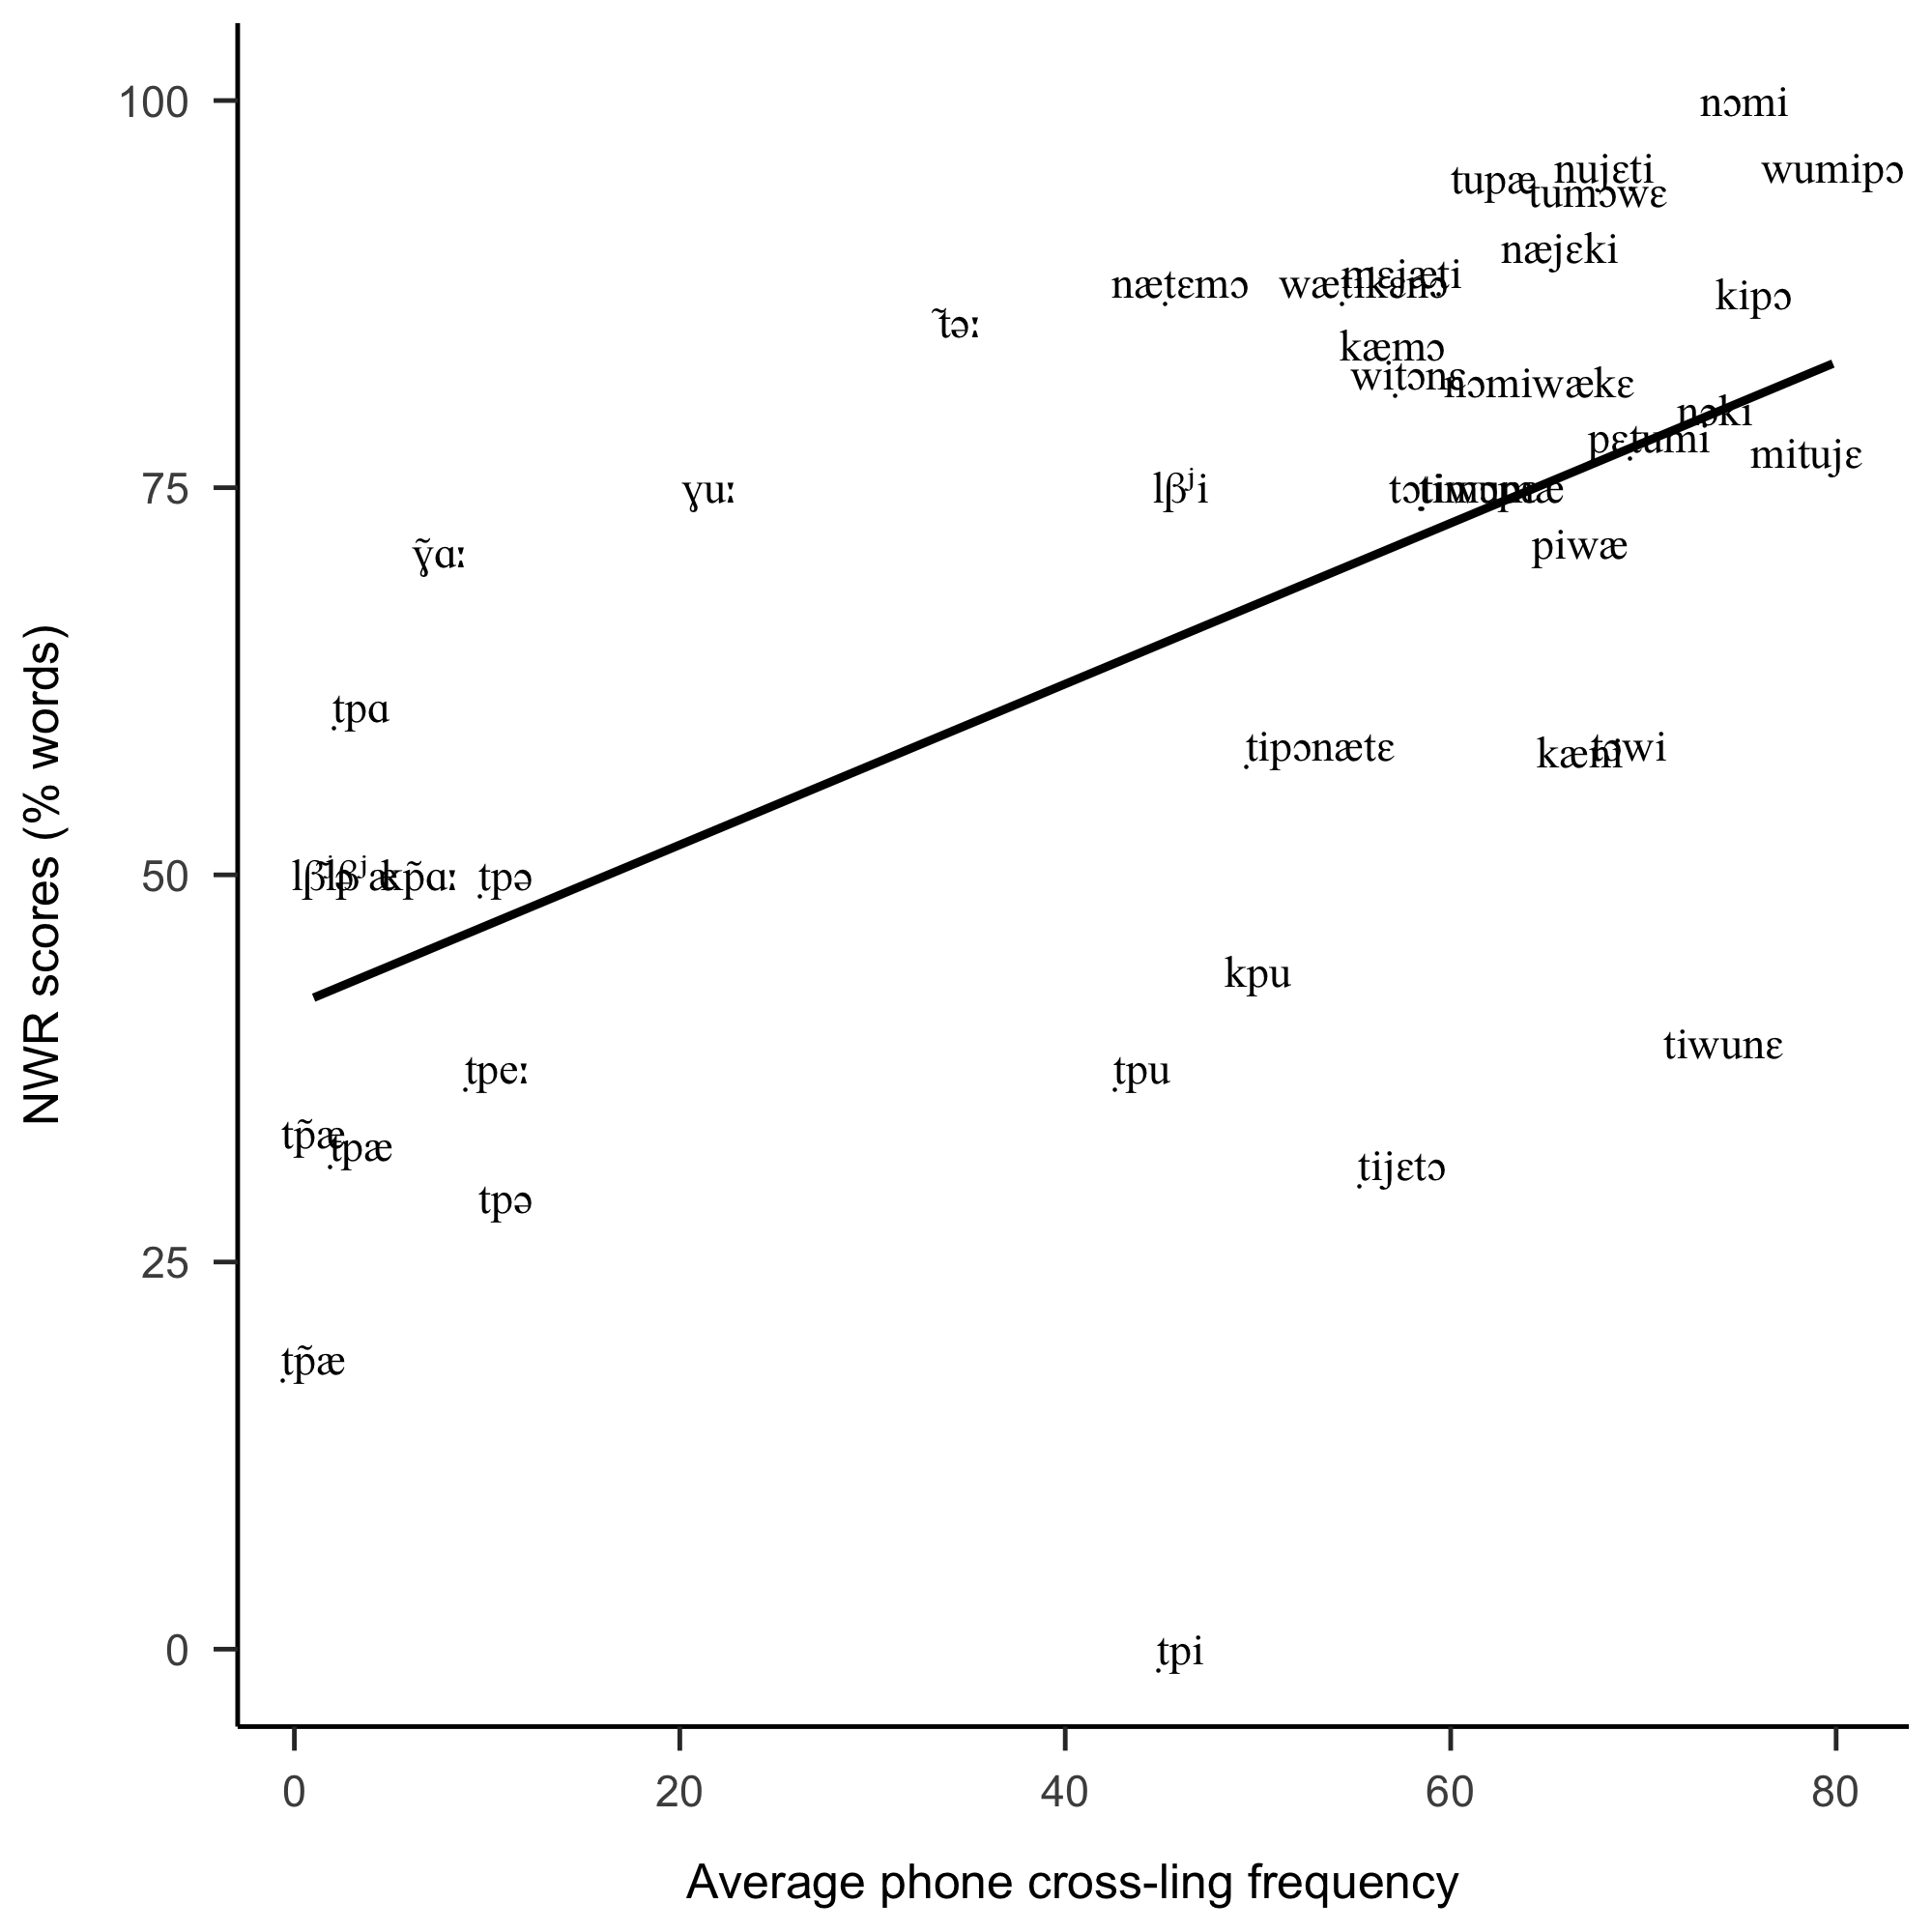
\includegraphics[width=0.65\linewidth]{nwr.by.freq.ITEM} 

}

\caption{NWR scores for individual target words as a function of the average frequency with which each phone is found across languages.}\label{fig:Fig2-xling-freq}
\end{figure}

We next checked whether this may actually be due to frequency of the sounds within the language. We estimated frequency of the phones present in the stimuli in a corpus of child-centered recordings (Casillas et al., 2020), and applied the natural logarithm. As before, unattested sounds were not considered (i.e., they were declared NA so that they do not count for analyses). Phone frequency estimated from this corpus were correlated with cross-linguistic phone frequencies (r(27)=0.52, =0.00). Therefore, we fit another mixed logistic regression, this time declaring as fixed effects scaled cross-linguistic and corpus frequencies (averaged across all attested phones within each stimulus item), in addition to age. As before, the model contained random slopes for both child ID and target. In this model, both cross-linguistic frequency (ß = 0.82, SE ß = 0.27, p = 0.00) and age (ß = 0.33, SE ß = 0.13, p = 0.01) were significant predictors of word-level NWR scores, but corpus frequency (ß = 0, SE ß = 0.25, p = 1.00) was not.

\textbf{use proportion of correctly produced rather than number; DONE}

\textbf{a2m use first attempts rather than the whole data set: having second thoughts. To be clear: the argument for using first attempts only is that all of the other analyses are on kids' first attempts, rather than all of their attempts, so we should use just first attempts here because it may confuse readers \& it is more consistent. BUT there are fewer mistakes this way, which is Options 1 and 2 below has lots of zeros\ldots{} CF Option 3 further down}

\textbf{a2m probably turn the paragraph on substitutions into a table: having second thoughts, the table would look just like a para, no?}

\textbf{Option 1: just numbers, first attempts only }
Next, we investigated patterns of deletion and substitution. Deletions were relatively rare, with only 7 vowels deleted, and 3 consonants.

As for substitutions, it was as common for a nasal vowel to be produced as an oral vowel as vice versa (34 oral target vowels produced as nasal vowels, 30 nasal target vowels produced as oral vowels). Substitutions in which the oral nature was preserved but the quality of the vowel was changed were a great deal more common than changes in quality among nasal vowels (110 oral vowels produced with a different quality; 13 nasal vowels produced with a different quality). As for consonants, asymmetries were very marked with more complex consonants (specifically dptpkpkmknmbghlv) mispronounced as simple ones (specifically mnlwyvdgptkfhch, 115) than vice versa (2). Simple consonants were mispronounced as other simple consonants quite frequently (69 simple consonants mispronounced as other simple ones, compared to 33 complex ones).

\textbf{Option 2: numbers and proportions, first attempts only}
Next, we investigated patterns of deletion and substitution. Deletions were relatively rare, with only 7 vowels deleted (about 0.23\% of all vowel targets), and 3 consonants deleted (about 0.12\% of all consonant targets).

As for substitutions, it was as common for a nasal vowel to be produced as an oral vowel as vice versa (34 oral target vowels produced as nasal vowels or about 0.99\% out of all oral vowel targets, 30 nasal target vowels produced as oral vowels or about 2.37\% out of all nasal vowel targets). Substitutions in which the oral nature was preserved but the quality of the vowel was changed were a great deal more common than changes in quality among nasal vowels (110 oral vowels produced with a different quality or about 1.86\% out of all oral vowel targets; 13 nasal vowels produced with a different quality or about 2.06\% out of all nasal vowel targets). As for consonants, asymmetries were very marked with more complex consonants (specifically dptpkpkmknmbghlv) mispronounced as simple ones (specifically mnlwyvdgptkfhch, 115 times or about 1.96\% out of all complex consonant targets) than vice versa (2 times or about 1.96\% out of all simple consonant targets). Simple consonants were mispronounced as other simple consonants quite frequently (69 simple consonants mispronounced as other simple ones or about 0.39\% out of all simple consonant targets, compared to 33 complex ones or about 1.02\% out of all complex consonant targets).

\textbf{Option 3: numbers and proportions, ALL attempts}
Next, we investigated patterns of deletion and substitution. Deletions were relatively rare, with only 12 vowels deleted (about 0.28\% of all vowel targets), and 6 consonants deleted (about 0.19\% of all consonant targets).

As for substitutions, it was as common for a nasal vowel to be produced as an oral vowel as vice versa (52 oral target vowels produced as nasal vowels or about 1.10\% out of all oral vowel targets, 58 nasal target vowels produced as oral vowels or about 2.53\% out of all nasal vowel targets). Substitutions in which the oral nature was preserved but the quality of the vowel was changed were a great deal more common than changes in quality among nasal vowels (205 oral vowels produced with a different quality or about 2.16\% out of all oral vowel targets; 23 nasal vowels produced with a different quality or about 2.36\% out of all nasal vowel targets). As for consonants, asymmetries were very marked with more complex consonants (specifically dptpkpkmknmbghlv) mispronounced as simple ones (specifically mnlwyvdgptkfhch, 250 times or about 2.43\% out of all complex consonant targets) than vice versa (2 times about 2.43\% out of all simple consonant targets). Simple consonants were mispronounced as other simple consonants quite frequently (123 simple consonants mispronounced as other simple ones or about 0.53\% out of all simple consonant targets, compared to 55 complex ones or about 0.98\% out of all complex consonant targets).

Finally, we looked into the frequency with which mispronunciations resulted in real words. Two thirds of them were: 62\%.

\hypertarget{nwr-scores-as-a-function-of-item-length}{%
\subsubsection{NWR scores as a function of item length}\label{nwr-scores-as-a-function-of-item-length}}

Next, we inspected whether NWR scores varied as a function of word length. Results are shown on table XX. This table shows that scores for monosyllables was much lower than for other lengths. This is likely due to the fact that the majority of monosyllables included were chosen because they had sounds that are rare in the world's languages, which may indicate that they are hard to produce or to perceive.

Setting monosyllables aside, we observe the typical pattern of lower scores for longer items, although this is particularly salient for the whole word scoring. This is the most commonly reported type of score, but it is also the least forgiving. The pattern is less marked when other two scores are used, which are less sensitive to errors.

\begin{table}[tbp]

\begin{center}
\begin{threeparttable}

\caption{\label{tab:tablength}NWR measured in whole-word scores, phoneme-based scores, and normalized Levenshtein Distance, separately for the four stimuli lengths.}

\begin{tabular}{lll}
\toprule
Word & \multicolumn{1}{c}{Phoneme} & \multicolumn{1}{c}{NLD}\\
\midrule
47 (22) & 59 (17) & 41 (17)\\
80 (22) & 93 (9) & 7 (9)\\
79 (19) & 93 (7) & 7 (7)\\
74 (32) & 91 (12) & 9 (12)\\
\bottomrule
\end{tabular}

\end{threeparttable}
\end{center}

\end{table}

\hypertarget{factor-structuring-individual-variation}{%
\subsubsection{Factor structuring individual variation}\label{factor-structuring-individual-variation}}

\begin{figure}
\centering
\includegraphics{manuscript_files/figure-latex/Fig2-scores by age-1.pdf}
\caption{(\#fig:Fig2-scores by age)NWR whole-word scores for individual participants as a function of age and sex (blue = boys, pink = girls).}
\end{figure}

Our final exploratory analysis assessed whether variation in scores was structured by factors that vary across individuals. As shown in Figure 2, there was a greater deal of variance in earlier than later ages, with significantly higher NWR scores for older children (Spearman's rank correlation, given inequality of variance, rho (6,496.39) = 0.43, p = 0.00). In contrast, there was no clear association between NWR scores, on the one hand, and sex (t (-0.61) = 27.83, p = 0.55), birth order (data missing for 17 children, rho = (2,652.32) = -0.15, p = 0.47) or maternal education (data missing for 2 children, rho = ( 9,022.76) = 0.09, p = 0.60).

\hypertarget{discussion}{%
\subsection{Discussion}\label{discussion}}

\begin{itemize}
\item
  What is the overall repetition scores (whole word, phoneme based, distance)?
\item
  How does this change as a function of item complexity (number of syllables, sound complexity)?
\end{itemize}

\begin{enumerate}
\def\labelenumi{\arabic{enumi}.}
\item
  Prediction based on previous work: Children have higher scores for shorter items
\item
  Prediction for Yélî made before seeing the data: The length distribution in Yélî words is more balanced than that in English, and thus the score decline for poly- versus mono-syllables may be less pronounced than that for English.
\item
  it turns out we were right! the scores for 2-4 syll words decline only slightly with length
\item
  Prediction based on previous work: Similarly, we do not know of NWR research that manipulates the difficulty of the sounds that are included in the items, but word naming and other research suggests that children achieve higher scores when producing easy and/or typologically common sounds than difficult and/or typologically rare sounds {[}CITE{]}. Therefore, we expect higher scores for items with common sounds than in those with rare sounds.
\item
  Prediction for Yélî made before seeing the data: The Yélî sound inventory is very large and compressed, with many similar sounds that are acoustic and articulatory neighbors. Therefore, this may constitute a pressure for children to have finer auditory skills (and perhaps more precise articulations) than children speaking languages with a simpler inventory. As a result, differences between easier and harder items may be smaller in this work than in other research.
\item
  it turns out we do see
\end{enumerate}

\textbf{(MC: but we can try and do a cursory analysis based on the corpora we have from Steve and my transcription of naturalistic interactions!)}

\begin{itemize}
\tightlist
\item
  How frequent are errors that result in real words? Is that a function of item complexity?
\item
  Is individual variation explainable by child age, sex, birth order, monolingual status, and/or parental education?
\end{itemize}

\begin{enumerate}
\def\labelenumi{\arabic{enumi}.}
\setcounter{enumi}{2}
\item
  Children's scores increases with child age.
\item
  General prediction: Non-monolingual Yélî children have lower scores than monolingual ones when tested on the society-dominant language (we did not test any non-dominant language)
\item
  Local prediction: Anecdotally Yélî children grow up in close-knitted communities and thus may receive significant portions of their language input from people not in their nuclear family
  (or at least from people other than their mothers, who tend to be the non-native speakers). If so, the difference between monolinguals and not monolinguals may be smaller than that found in other work
  . That said, one recent study on the same population shows that most child-directed input in the first 2 years does come from the mother
  , so in so far as this input has a crucial formational role, then there may still be a score difference between these two groups.
\item
  We don't see a difference
\item
  General prediction: previous NWR evidence on this is mixed, but general findings on language development suggest that children whose mothers are more educated score higher in standardized language tests (eg ppvt) than children whose mothers are less educated.
\item
  Prediction made before seeing data: In the Rossel community, formal education plays an extremely minor role in ensuring individual's success, is not a good index of relative socio-economic status, and furthermore there is only a narrow range of variation in maternal educational attainment. This may lead to no or only very small advantages for children whose mothers are more educated, provided that the causal chain between maternal education and child language is via SES more broadly. However, if education directly boosts maternal verbal skills and the incidence of verbal behavior (as suggested by CITE), then we should still see a difference along this factor.
\item
  We did not find this
\item
  General prediction: To our knowledge, there is no previous NWR work on this, but other research suggests that first-born children score higher in standardized language tests later-born children.
\item
  Prediction before seeing data: One main causal path between birth order and language development is via parental input (CITE). Given our arguments above for how mothers may not be as important among Rossel people than in other places, then the difference in scores between first borns and later borns may be small
\item
  we did not find a sig effect, but this is a small effect (eg d=.2 in Havron et al)
\end{enumerate}

\newpage

\hypertarget{acknowledgments}{%
\subsection{Acknowledgments}\label{acknowledgments}}

We are grateful to the individuals who participated in the study. The collection and annotation of these recordings was made possible by Ndapw:éé Yidika, Taakêmê Ńamono, and Y:aaw:aa Pikuwa; with thanks also to the PNG National Research Institute, and the Administration of Milne Bay Province AC acknowledges financial and institutional support from Agence Nationale de la Recherche (ANR-17-CE28-0007 LangAge, ANR-16-DATA-0004 ACLEW, ANR-14-CE30-0003 MechELex, ANR-17-EURE-0017) and the J. S. McDonnell Foundation Understanding Human Cognition Scholar Award. MC acknowledges financial support from an NWO Veni Innovational Scheme grant (275-89-033).

\hypertarget{references}{%
\section{References}\label{references}}

\setlength{\parindent}{-0.5in}
\setlength{\leftskip}{0.5in}

\hypertarget{refs}{}
\leavevmode\hypertarget{ref-is08042009language}{}%
Action, C. (2009). Language impairment in a multilingual society: Linguistic patterns and the road to assessment. \emph{Brussels: COST Office. Available Online at: Http://Www. Bi-Sli. Org}.

\leavevmode\hypertarget{ref-balladares2016socio}{}%
Balladares, J., Marshall, C., \& Griffiths, Y. (2016). Socio-economic status affects sentence repetition, but not non-word repetition, in Chilean preschoolers. \emph{First Language}, \emph{36}(3), 338--351. \url{https://doi.org/10.1177/0142723715626067}

\leavevmode\hypertarget{ref-bergelsoncasillas2019what}{}%
Bergelson, E., Casillas, M., Soderstrom, M., Seidl, A., Warlaumont, A. S., \& Amatuni, A. (2019). What do North American babies hear? A large-scale cross-corpus analysis. \emph{Developmental Science}, \emph{22}(1), e12724. \url{https://doi.org/10.1111/desc.12724}

\leavevmode\hypertarget{ref-bowey2001nonword}{}%
Bowey, J. A. (2001). Nonword repetition and young children's receptive vocabulary: A longitudinal study. \emph{Applied Psycholinguistics}, \emph{22}(3), 441--469.

\leavevmode\hypertarget{ref-brandeker2015language}{}%
Brandeker, M., \& Thordardottir, E. (2015). Language exposure in bilingual toddlers: Performance on nonword repetition and lexical tasks. \emph{American Journal of Speech-Language Pathology}, \emph{24}(2), 126--138.

\leavevmode\hypertarget{ref-brown2011cultural}{}%
Brown, P. (2011). The cultural organization of attention. In A. Duranti, E. Ochs, \& and Bambi B Schieffelin (Eds.), \emph{Handbook of Language Socialization} (pp. 29--55). Malden, MA: Wiley-Blackwell.

\leavevmode\hypertarget{ref-brown2014interactional}{}%
Brown, P. (2014). The interactional context of language learning in Tzeltal. In I. Arnon, M. Casillas, C. Kurumada, \& B. Estigarribia (Eds.), \emph{Language in interaction: Studies in honor of Eve V. Clark} (pp. 51--82). Amsterdam, NL: John Benjamins.

\leavevmode\hypertarget{ref-brownIPchildrearing}{}%
Brown, P., \& Casillas, M. (n.d.). Childrearing through social interaction on Rossel Island, PNG. In A. J. Fentiman \& M. Goody (Eds.), \emph{Esther Goody revisited: Exploring the legacy of an original inter-disciplinarian} (pp. XX--XX). New York, NY: Berghahn.

\leavevmode\hypertarget{ref-bunceURcrosscultural}{}%
Bunce, J., Soderstrom, M., Bergelson, E., Rosemberg, C., Stein, A., Alam, F., \ldots{} Casillas, M. (n.d.). A cross-cultural examination of young children's everyday language experiences.

\leavevmode\hypertarget{ref-casillas2020early}{}%
Casillas, M., Brown, P., \& Levinson, S. C. (2020). Early language experience in a papuan community. \emph{Journal of Child Language}, \emph{XX}, XX--XX.

\leavevmode\hypertarget{ref-chiat2007preschool}{}%
Chiat, S., \& Roy, P. (2007). The preschool repetition test: An evaluation of performance in typically developing and clinically referred children. \emph{Journal of Speech, Language, and Hearing Research}, \emph{50}(2), 429--443.

\leavevmode\hypertarget{ref-cristia2020infant}{}%
Cristia, A., Farabolini, G., Scaff, C., Havron, N., \& Stieglitz, J. (2020). Infant-directed input and literacy effects on phonological processing: Non-word repetition scores among the tsimane'. \emph{Preprint}.

\leavevmode\hypertarget{ref-estes2007differences}{}%
Estes, K. G., Evans, J. L., \& Else-Quest, N. M. (2007). Differences in the nonword repetition performance of children with and without specific language impairment: A meta-analysis. \emph{Journal of Speech, Language, and Hearing Research}, \emph{50}(1), 177--195.

\leavevmode\hypertarget{ref-farmani2018normalization}{}%
Farmani, H., Sayyahi, F., Soleymani, Z., Labbaf, F. Z., Talebi, E., \& Shourvazi, Z. (2018). Normalization of the non-word repetition test in farsi-speaking children. \emph{Journal of Modern Rehabilitation}, \emph{12}(4), 217--224.

\leavevmode\hypertarget{ref-gallagher2014identity}{}%
Gallagher, G. (2014). An identity bias in phonotactics: Evidence from Cochabamba Quechua. \emph{Laboratory Phonology}, \emph{5}(3), 337--378. \url{https://doi.org/10.1515/lp-2014-0012}

\leavevmode\hypertarget{ref-gallon2007non}{}%
Gallon, N., Harris, J., \& Van der Lely, H. (2007). Non-word repetition: An investigation of phonological complexity in children with grammatical sli. \emph{Clinical Linguistics \& Phonetics}, \emph{21}(6), 435--455.

\leavevmode\hypertarget{ref-havron2019effect}{}%
Havron, N., Ramus, F., Heude, B., Forhan, A., Cristia, A., Peyre, H., \& Group, E. M.-C. C. S. (2019). The effect of older siblings on language development as a function of age difference and sex. \emph{Psychological Science}, \emph{30}(9), 1333--1343.

\leavevmode\hypertarget{ref-hazan2000development}{}%
Hazan, V., \& Barrett, S. (2000). The development of phonemic categorization in children aged 6--12. \emph{Journal of Phonetics}, \emph{28}(4), 377--396.

\leavevmode\hypertarget{ref-jabere2018xperiment}{}%
Jaber-Awida, A. (2018). Experiment in non word repetition by monolingual Arabic preschoolers. \emph{Athens Journal of Philology}, \emph{5}(4), 317--334. \url{https://doi.org/10.30958/ajp.5-4-4}

\leavevmode\hypertarget{ref-kalnak2014nonword}{}%
Kalnak, N., Peyrard-Janvid, M., Forssberg, H., \& Sahlén, B. (2014). Nonword repetition--a clinical marker for specific language impairment in swedish associated with parents' language-related problems. \emph{PloS One}, \emph{9}(2), e89544.

\leavevmode\hypertarget{ref-levinsoninprepydgrammar}{}%
Levinson, S. C. (n.d.). \emph{A grammar of yélî dnye, the papuan language of rossel island}. Cambridge, UK: Cambridge University Press.

\leavevmode\hypertarget{ref-liszkowski2012prelinguistic}{}%
Liszkowski, U., Brown, P., Callaghan, T., Takada, A., \& de Vos, C. (2012). A prelinguistic gestural universal of human communication. \emph{Cognitive Science}, \emph{36}(4), 698--713. \url{https://doi.org/10.1111/j.1551-6709.2011.01228.x}

\leavevmode\hypertarget{ref-meir2017independent}{}%
Meir, N., \& Armon-Lotem, S. (2017). Independent and combined effects of socioeconomic status (ses) and bilingualism on children's vocabulary and verbal short-term memory. \emph{Frontiers in Psychology}, \emph{8}, 1442.

\leavevmode\hypertarget{ref-meir2016disentangling}{}%
Meir, N., Walters, J., \& Armon-Lotem, S. (2016). Disentangling sli and bilingualism using sentence repetition tasks: The impact of l1 and l2 properties. \emph{International Journal of Bilingualism}, \emph{20}(4), 421--452.

\leavevmode\hypertarget{ref-phoible}{}%
Moran, S., \& McCloy, D. (Eds.). (2019). \emph{PHOIBLE 2.0}. Jena: Max Planck Institute for the Science of Human History. Retrieved from \url{https://phoible.org/}

\leavevmode\hypertarget{ref-piazzalunga2019articulatory}{}%
Piazzalunga, S., Previtali, L., Pozzoli, R., Scarponi, L., \& Schindler, A. (2019). An articulatory-based disyllabic and trisyllabic non-word repetition test: Reliability and validity in italian 3-to 7-year-old children. \emph{Clinical Linguistics \& Phonetics}, \emph{33}(5), 437--456.

\leavevmode\hypertarget{ref-torrington2015non}{}%
Torrington Eaton, C., Newman, R. S., Ratner, N. B., \& Rowe, M. L. (2015). Non-word repetition in 2-year-olds: Replication of an adapted paradigm and a useful methodological extension. \emph{Clinical Linguistics \& Phonetics}, \emph{29}(7), 523--535.

\leavevmode\hypertarget{ref-vance2005speech}{}%
Vance, M., Stackhouse, J., \& Wells, B. (2005). Speech-production skills in children aged 3--7 years. \emph{International Journal of Language \& Communication Disorders}, \emph{40}(1), 29--48.

\leavevmode\hypertarget{ref-wilsenach2013phonological}{}%
Wilsenach, C. (2013). Phonological skills as predictor of reading success: An investigation of emergent bilingual Northern Sotho/English learners. \emph{Per Linguam: a Journal of Language Learning= Per Linguam: Tydskrif vir Taalaanleer}, \emph{29}(2), 17--32. \url{https://doi.org/10.5785/29-2-554}

\leavevmode\hypertarget{ref-is08042009language}{}%
Action, C. (2009). Language impairment in a multilingual society: Linguistic patterns and the road to assessment. \emph{Brussels: COST Office. Available Online at: Http://Www. Bi-Sli. Org}.

\leavevmode\hypertarget{ref-balladares2016socio}{}%
Balladares, J., Marshall, C., \& Griffiths, Y. (2016). Socio-economic status affects sentence repetition, but not non-word repetition, in Chilean preschoolers. \emph{First Language}, \emph{36}(3), 338--351. \url{https://doi.org/10.1177/0142723715626067}

\leavevmode\hypertarget{ref-bergelsoncasillas2019what}{}%
Bergelson, E., Casillas, M., Soderstrom, M., Seidl, A., Warlaumont, A. S., \& Amatuni, A. (2019). What do North American babies hear? A large-scale cross-corpus analysis. \emph{Developmental Science}, \emph{22}(1), e12724. \url{https://doi.org/10.1111/desc.12724}

\leavevmode\hypertarget{ref-bowey2001nonword}{}%
Bowey, J. A. (2001). Nonword repetition and young children's receptive vocabulary: A longitudinal study. \emph{Applied Psycholinguistics}, \emph{22}(3), 441--469.

\leavevmode\hypertarget{ref-brandeker2015language}{}%
Brandeker, M., \& Thordardottir, E. (2015). Language exposure in bilingual toddlers: Performance on nonword repetition and lexical tasks. \emph{American Journal of Speech-Language Pathology}, \emph{24}(2), 126--138.

\leavevmode\hypertarget{ref-brown2011cultural}{}%
Brown, P. (2011). The cultural organization of attention. In A. Duranti, E. Ochs, \& and Bambi B Schieffelin (Eds.), \emph{Handbook of Language Socialization} (pp. 29--55). Malden, MA: Wiley-Blackwell.

\leavevmode\hypertarget{ref-brown2014interactional}{}%
Brown, P. (2014). The interactional context of language learning in Tzeltal. In I. Arnon, M. Casillas, C. Kurumada, \& B. Estigarribia (Eds.), \emph{Language in interaction: Studies in honor of Eve V. Clark} (pp. 51--82). Amsterdam, NL: John Benjamins.

\leavevmode\hypertarget{ref-brownIPchildrearing}{}%
Brown, P., \& Casillas, M. (n.d.). Childrearing through social interaction on Rossel Island, PNG. In A. J. Fentiman \& M. Goody (Eds.), \emph{Esther Goody revisited: Exploring the legacy of an original inter-disciplinarian} (pp. XX--XX). New York, NY: Berghahn.

\leavevmode\hypertarget{ref-bunceURcrosscultural}{}%
Bunce, J., Soderstrom, M., Bergelson, E., Rosemberg, C., Stein, A., Alam, F., \ldots{} Casillas, M. (n.d.). A cross-cultural examination of young children's everyday language experiences.

\leavevmode\hypertarget{ref-casillas2020early}{}%
Casillas, M., Brown, P., \& Levinson, S. C. (2020). Early language experience in a papuan community. \emph{Journal of Child Language}, \emph{XX}, XX--XX.

\leavevmode\hypertarget{ref-chiat2007preschool}{}%
Chiat, S., \& Roy, P. (2007). The preschool repetition test: An evaluation of performance in typically developing and clinically referred children. \emph{Journal of Speech, Language, and Hearing Research}, \emph{50}(2), 429--443.

\leavevmode\hypertarget{ref-cristia2020infant}{}%
Cristia, A., Farabolini, G., Scaff, C., Havron, N., \& Stieglitz, J. (2020). Infant-directed input and literacy effects on phonological processing: Non-word repetition scores among the tsimane'. \emph{Preprint}.

\leavevmode\hypertarget{ref-estes2007differences}{}%
Estes, K. G., Evans, J. L., \& Else-Quest, N. M. (2007). Differences in the nonword repetition performance of children with and without specific language impairment: A meta-analysis. \emph{Journal of Speech, Language, and Hearing Research}, \emph{50}(1), 177--195.

\leavevmode\hypertarget{ref-farmani2018normalization}{}%
Farmani, H., Sayyahi, F., Soleymani, Z., Labbaf, F. Z., Talebi, E., \& Shourvazi, Z. (2018). Normalization of the non-word repetition test in farsi-speaking children. \emph{Journal of Modern Rehabilitation}, \emph{12}(4), 217--224.

\leavevmode\hypertarget{ref-gallagher2014identity}{}%
Gallagher, G. (2014). An identity bias in phonotactics: Evidence from Cochabamba Quechua. \emph{Laboratory Phonology}, \emph{5}(3), 337--378. \url{https://doi.org/10.1515/lp-2014-0012}

\leavevmode\hypertarget{ref-gallon2007non}{}%
Gallon, N., Harris, J., \& Van der Lely, H. (2007). Non-word repetition: An investigation of phonological complexity in children with grammatical sli. \emph{Clinical Linguistics \& Phonetics}, \emph{21}(6), 435--455.

\leavevmode\hypertarget{ref-havron2019effect}{}%
Havron, N., Ramus, F., Heude, B., Forhan, A., Cristia, A., Peyre, H., \& Group, E. M.-C. C. S. (2019). The effect of older siblings on language development as a function of age difference and sex. \emph{Psychological Science}, \emph{30}(9), 1333--1343.

\leavevmode\hypertarget{ref-hazan2000development}{}%
Hazan, V., \& Barrett, S. (2000). The development of phonemic categorization in children aged 6--12. \emph{Journal of Phonetics}, \emph{28}(4), 377--396.

\leavevmode\hypertarget{ref-jabere2018xperiment}{}%
Jaber-Awida, A. (2018). Experiment in non word repetition by monolingual Arabic preschoolers. \emph{Athens Journal of Philology}, \emph{5}(4), 317--334. \url{https://doi.org/10.30958/ajp.5-4-4}

\leavevmode\hypertarget{ref-kalnak2014nonword}{}%
Kalnak, N., Peyrard-Janvid, M., Forssberg, H., \& Sahlén, B. (2014). Nonword repetition--a clinical marker for specific language impairment in swedish associated with parents' language-related problems. \emph{PloS One}, \emph{9}(2), e89544.

\leavevmode\hypertarget{ref-levinsoninprepydgrammar}{}%
Levinson, S. C. (n.d.). \emph{A grammar of yélî dnye, the papuan language of rossel island}. Cambridge, UK: Cambridge University Press.

\leavevmode\hypertarget{ref-liszkowski2012prelinguistic}{}%
Liszkowski, U., Brown, P., Callaghan, T., Takada, A., \& de Vos, C. (2012). A prelinguistic gestural universal of human communication. \emph{Cognitive Science}, \emph{36}(4), 698--713. \url{https://doi.org/10.1111/j.1551-6709.2011.01228.x}

\leavevmode\hypertarget{ref-meir2017independent}{}%
Meir, N., \& Armon-Lotem, S. (2017). Independent and combined effects of socioeconomic status (ses) and bilingualism on children's vocabulary and verbal short-term memory. \emph{Frontiers in Psychology}, \emph{8}, 1442.

\leavevmode\hypertarget{ref-meir2016disentangling}{}%
Meir, N., Walters, J., \& Armon-Lotem, S. (2016). Disentangling sli and bilingualism using sentence repetition tasks: The impact of l1 and l2 properties. \emph{International Journal of Bilingualism}, \emph{20}(4), 421--452.

\leavevmode\hypertarget{ref-phoible}{}%
Moran, S., \& McCloy, D. (Eds.). (2019). \emph{PHOIBLE 2.0}. Jena: Max Planck Institute for the Science of Human History. Retrieved from \url{https://phoible.org/}

\leavevmode\hypertarget{ref-piazzalunga2019articulatory}{}%
Piazzalunga, S., Previtali, L., Pozzoli, R., Scarponi, L., \& Schindler, A. (2019). An articulatory-based disyllabic and trisyllabic non-word repetition test: Reliability and validity in italian 3-to 7-year-old children. \emph{Clinical Linguistics \& Phonetics}, \emph{33}(5), 437--456.

\leavevmode\hypertarget{ref-torrington2015non}{}%
Torrington Eaton, C., Newman, R. S., Ratner, N. B., \& Rowe, M. L. (2015). Non-word repetition in 2-year-olds: Replication of an adapted paradigm and a useful methodological extension. \emph{Clinical Linguistics \& Phonetics}, \emph{29}(7), 523--535.

\leavevmode\hypertarget{ref-vance2005speech}{}%
Vance, M., Stackhouse, J., \& Wells, B. (2005). Speech-production skills in children aged 3--7 years. \emph{International Journal of Language \& Communication Disorders}, \emph{40}(1), 29--48.

\leavevmode\hypertarget{ref-wilsenach2013phonological}{}%
Wilsenach, C. (2013). Phonological skills as predictor of reading success: An investigation of emergent bilingual Northern Sotho/English learners. \emph{Per Linguam: a Journal of Language Learning= Per Linguam: Tydskrif vir Taalaanleer}, \emph{29}(2), 17--32. \url{https://doi.org/10.5785/29-2-554}

\end{document}
